% WACV 2027 Paper Template (official author kit, wacv.thecvf.com/static/wacv-2027-author-kit-template.zip)
\documentclass[10pt,twocolumn,letterpaper]{article}

%%%%%%%%% PAPER TYPE
% HARVEST-Vision 2027 uses SINGLE-BLIND review (author names must appear), so we use the
% camera-ready format with page numbers instead of the anonymous [review] option.
\usepackage[pagenumbers]{wacv}

%
% --- inline annotations
%
\newcommand{\red}[1]{{\color{red}#1}}
\newcommand{\todo}[1]{{\color{red}#1}}
\newcommand{\TODO}[1]{\textbf{\color{red}[TODO: #1]}}
% --- disable by uncommenting  
% \renewcommand{\TODO}[1]{}
% \renewcommand{\todo}[1]{#1}



\usepackage{booktabs}
\usepackage{graphicx}
\usepackage{amsmath}
\usepackage{xspace}
\xspaceaddexceptions{]\%}
\usepackage{caption}
\definecolor{wacvblue}{rgb}{0.21,0.49,0.74}
\usepackage[pagebackref,breaklinks,colorlinks,allcolors=wacvblue]{hyperref}

\def\wacvPaperID{*****}
\def\confName{WACV}
\def\confYear{2027}

\newcommand{\NumRuns}{67\xspace}
\newcommand{\GPUHours}{1.8\xspace}
\newcommand{\PDdups}{27\xspace}
\newcommand{\PDtestN}{236\xspace}
\newcommand{\PVtrainN}{30978\xspace}
\newcommand{\PVtestN}{7564\xspace}
\newcommand{\PDtrainN}{2334\xspace}
\newcommand{\ClipPD}{29.2\xspace}
\newcommand{\ClipPV}{25.2\xspace}
\newcommand{\mnvthreepvpre}{30.9\xspace}
\newcommand{\mnvthreepdkfiveinit}{40.0\xspace}
\newcommand{\mnvthreepdallinit}{66.8\xspace}
\newcommand{\mnvthreepdkfivepre}{25.1\xspace}
\newcommand{\mnvthreepdallpre}{57.3\xspace}
\newcommand{\mnvthreePVin}{98.9\xspace}
\newcommand{\mnvthreeGap}{67.9\xspace}
\newcommand{\mnvthreeSeedSD}{1.9\xspace}
\newcommand{\effbzeropvpre}{31.9\xspace}
\newcommand{\effbzeropdkfiveinit}{39.1\xspace}
\newcommand{\effbzeropdallinit}{65.3\xspace}
\newcommand{\effbzeropdkfivepre}{25.1\xspace}
\newcommand{\effbzeropdallpre}{59.5\xspace}
\newcommand{\effbzeroPVin}{99.4\xspace}
\newcommand{\effbzeroGap}{67.5\xspace}
\newcommand{\effbzeroSeedSD}{2.4\xspace}
\newcommand{\dinovtwoslppvpre}{46.2\xspace}
\newcommand{\dinovtwoslppdkfiveinit}{55.4\xspace}
\newcommand{\dinovtwoslppdallinit}{67.8\xspace}
\newcommand{\dinovtwoslppdkfivepre}{45.1\xspace}
\newcommand{\dinovtwoslppdallpre}{73.0\xspace}
\newcommand{\dinovtwoslpPVin}{97.6\xspace}
\newcommand{\dinovtwoslpGap}{51.4\xspace}
\newcommand{\dinovtwoslpSeedSD}{1.7\xspace}
\newcommand{\dinovtwosftpvpre}{37.7\xspace}
\newcommand{\dinovtwosftpdkfiveinit}{52.4\xspace}
\newcommand{\dinovtwosftpdallinit}{72.7\xspace}
\newcommand{\dinovtwosftpdkfivepre}{39.8\xspace}
\newcommand{\dinovtwosftpdallpre}{72.9\xspace}
\newcommand{\dinovtwosftPVin}{99.5\xspace}
\newcommand{\dinovtwosftGap}{61.8\xspace}
\newcommand{\dinovtwosftSeedSD}{2.2\xspace}
\newcommand{\EdgeCPU}{AMD Ryzen 7 9800X3D 8-Core Processor\xspace}
\newcommand{\CPUfourMnv}{0.9\xspace}
\newcommand{\CPUoneMnv}{2.7\xspace}
\newcommand{\ParamsMnv}{4.2\xspace}
\newcommand{\CPUfourEff}{1.9\xspace}
\newcommand{\CPUoneEff}{5.3\xspace}
\newcommand{\ParamsEff}{4.0\xspace}
\newcommand{\CPUfourDino}{18.1\xspace}
\newcommand{\CPUoneDino}{51.8\xspace}
\newcommand{\ParamsDino}{21.6\xspace}
% DINOv2-LP vs EfficientNet-B0 (PV only)
\newcommand{\PCa}{+14.3\xspace}
\newcommand{\PCalo}{+8.2\xspace}
\newcommand{\PCahi}{+20.2\xspace}
% DINOv2-LP vs DINOv2-FT (PV only)
\newcommand{\PCb}{+8.5\xspace}
\newcommand{\PCblo}{+3.1\xspace}
\newcommand{\PCbhi}{+13.6\xspace}
% DINOv2-LP (PV only) vs CLIP zero-shot
\newcommand{\PCc}{+16.9\xspace}
\newcommand{\PCclo}{+8.1\xspace}
\newcommand{\PCchi}{+25.3\xspace}
% MobileNetV3-L: PV→5/class vs 5/class only
\newcommand{\PCd}{+14.8\xspace}
\newcommand{\PCdlo}{+10.7\xspace}
\newcommand{\PCdhi}{+19.1\xspace}
% MobileNetV3-L: PV→all vs all field only
\newcommand{\PCe}{+9.5\xspace}
\newcommand{\PCelo}{+5.6\xspace}
\newcommand{\PCehi}{+13.3\xspace}
% EfficientNet-B0: PV→5/class vs 5/class only
\newcommand{\PCf}{+14.0\xspace}
\newcommand{\PCflo}{+10.2\xspace}
\newcommand{\PCfhi}{+17.9\xspace}
% EfficientNet-B0: PV→all vs all field only
\newcommand{\PCg}{+5.8\xspace}
\newcommand{\PCglo}{+2.3\xspace}
\newcommand{\PCghi}{+9.3\xspace}
% DINOv2 ViT-S/14 (linear probe): PV→5/class vs 5/class only
\newcommand{\PCh}{+10.3\xspace}
\newcommand{\PChlo}{+5.6\xspace}
\newcommand{\PChhi}{+14.8\xspace}
% DINOv2 ViT-S/14 (linear probe): PV→all vs all field only
\newcommand{\PCi}{-5.2\xspace}
\newcommand{\PCilo}{-8.8\xspace}
\newcommand{\PCihi}{-2.0\xspace}
% DINOv2 ViT-S/14 (fine-tune): PV→5/class vs 5/class only
\newcommand{\PCj}{+12.6\xspace}
\newcommand{\PCjlo}{+8.3\xspace}
\newcommand{\PCjhi}{+16.9\xspace}
% DINOv2 ViT-S/14 (fine-tune): PV→all vs all field only
\newcommand{\PCk}{-0.1\xspace}
\newcommand{\PCklo}{-3.1\xspace}
\newcommand{\PCkhi}{+3.0\xspace}
\newcommand{\mnvthreeRec}{25\xspace}
\newcommand{\effbzeroRec}{22\xspace}
\newcommand{\dinovtwoslpRec}{42\xspace}
\newcommand{\dinovtwosftRec}{42\xspace}
\newcommand{\CIhwMin}{5.7\xspace}
\newcommand{\CIhwMax}{6.4\xspace}
\newcommand{\HealthyMajority}{61.9\xspace}
\newcommand{\CropAccMnv}{53.8\xspace}
\newcommand{\ClassGivenCropMnv}{57.5\xspace}
\newcommand{\CropAccEff}{55.9\xspace}
\newcommand{\ClassGivenCropEff}{57.2\xspace}
\newcommand{\CropAccLP}{74.6\xspace}
\newcommand{\ClassGivenCropLP}{61.9\xspace}
\newcommand{\CropAccFT}{64.8\xspace}
\newcommand{\ClassGivenCropFT}{58.2\xspace}

\newcommand{\PV}{PlantVillage\xspace}
\newcommand{\PD}{PlantDoc\xspace}

\title{Lab-to-Field on a Budget: A Seeded, Edge-Aware Benchmark of\\Plant Disease Classifiers under the PlantVillage$\rightarrow$PlantDoc Shift}

%%%%%%%%% AUTHORS -- TO BE FILLED IN BY THE AUTHORS (single-blind venue)
\author{Johnathan Luu \qquad Aryan Padarthi\\
Allen High School\\
{\tt\small \{johnathan.luu, aryan.padarthi\}@student.allenisd.org}
}

\begin{document}
\maketitle
\begin{abstract}
Plant-disease classifiers routinely exceed 99\% accuracy on the PlantVillage lab dataset, yet published numbers on field images vary widely and are rarely reproducible.
We release a small, fully seeded benchmark of the PlantVillage$\rightarrow$PlantDoc shift. It has a fixed one-to-one 28-class label map, leaf-grouped source splits, a near-duplicate audit of the target test set, three seeds per configuration, bootstrap confidence intervals, and CPU/GPU cost measurements.
We compare two edge CNNs (MobileNetV3, EfficientNet-B0), a DINOv2 ViT-S as a frozen linear probe or fine-tuned, and CLIP zero-shot, under five label regimes ranging from no field labels to the full PlantDoc training set.
Every lab-trained model loses \dinovtwoslpGap--\mnvthreeGap\ points on field images.
A frozen DINOv2 probe trained only on lab images is the strongest source-only model (\PCa\ points over EfficientNet-B0, paired 95\% CI [\PCalo, \PCahi]), and it beats fine-tuning the same backbone.
Five field images per class recover only \effbzeroRec--\dinovtwoslpRec\% of the gap to full field supervision, which falsifies one of our pre-registered claims.
Lab pretraining helps the CNNs at every label budget we tested. For DINOv2 it helps only when field labels are scarce: once all field labels are available it is neutral for fine-tuning, and a lab-trained head initialization \emph{hurts} the frozen probe.
The \PDtestN-image PlantDoc test set also limits what can be concluded: 95\% bootstrap intervals span $\pm$\CIhwMin--\CIhwMax\ points, about three times the seed-to-seed standard deviation, and \PDdups test images are near-duplicates of training images.
The whole study used \GPUHours\ GPU-hours. Code, configs, logs and per-run predictions are released at \url{https://github.com/Edtwo/lab-to-field-plant-disease}.
\end{abstract}

\section{Introduction}
\label{sec:intro}

Image-based disease diagnosis is one of the most-cited use cases of computer vision in agriculture. It is also one of the clearest examples of a benchmark that has outrun deployment.
Models trained on \PV~\cite{hughes2015an}, whose leaves are photographed one at a time on uniform backgrounds, reach about 99\% held-out accuracy~\cite{mohanty2016using}. On photos taken in real fields~\cite{singh2020plantdoc}, the same models do far worse.
Recent work attacks this gap with larger and more specialized models~\cite{salman2025plant,mooraj2026agripath,mamun2025psmamba}. But the numbers being compared are hard to interpret. Label mappings between datasets are rarely published, results usually come from a single run, small field test sets are reported without intervals, and the compute or latency needed in the field is seldom measured.

This paper takes a deliberately modest position. Before proposing new methods for lab-to-field transfer, we should be able to measure it reproducibly, with honest uncertainty, under a compute budget a typical agricultural lab or extension service can afford.
We build such a measurement for the most widely used pair, \PV$\rightarrow$\PD, and use it to ask three practical questions:
\begin{enumerate}
\item How much does generic self-supervised pretraining help compared with small supervised CNNs when \emph{no} field labels exist?
\item How much do a \emph{handful} of field labels (5 per class) buy, compared with all available field labels?
\item Is lab data worth using at all once field labels exist, and does the answer depend on the model?
\end{enumerate}

\paragraph{Contributions.}
\begin{itemize}
\item A released, seeded protocol for \PV$\rightarrow$\PD: a one-to-one 28-class label map, leaf-grouped source splits, a near-duplicate audit (\PDdups of \PDtestN \PD test images duplicate training images), three seeds, bootstrap and paired-bootstrap intervals, and CPU/GPU cost. The full study takes \GPUHours GPU-hours on one consumer GPU (\cref{sec:method,sec:setup}).
\item Five claims pre-registered with numeric thresholds before any results came in. Three hold and two are falsified, and we report both (\cref{sec:results}).
\item Two findings practitioners can act on (\cref{sec:results}). First, a \emph{frozen} DINOv2 ViT-S probe trained only on lab images beats both fine-tuned edge CNNs and fine-tuned DINOv2 on field images. Second, lab pretraining helps CNNs at every label budget we tested. For DINOv2, its value disappears (fine-tuning) or turns negative (lab-trained head for the frozen probe) once all field labels are available.
\item A quantified caution: on \PD, test-set sampling noise ($\pm$\CIhwMin--\CIhwMax\ points) is larger than seed noise, so many published single-number comparisons on this split cannot be distinguished (\cref{sec:limits}).
\end{itemize}

\section{Related Work}
\label{sec:related}

\paragraph{Lab-to-field shift.}
\PV~\cite{hughes2015an} made large-scale leaf-disease classification possible. Mohanty \etal~\cite{mohanty2016using} reported 99.35\% held-out accuracy on it. The arXiv version of the same study also reports only 31.4\% on images from other sources.
\PD~\cite{singh2020plantdoc} collected 2.6k in-the-wild images of 13 crops for exactly this reason. Since then, lab-to-field transfer has been tackled with mixture-of-experts ViTs~\cite{salman2025plant}, cross-domain few-shot learning~\cite{yang2024laboratory}, CLIP-style zero-shot transfer~\cite{benabbas2025rethinking}, and comparisons of CNNs with contrastive and generative VLMs~\cite{mooraj2026agripath}.
Xu \etal argue that strong benchmark numbers are partly an artifact of how the datasets were built~\cite{xu2023plant,xu2023embrace}.
Published \PV$\rightarrow$\PD accuracies range widely: 48\% for ViT-B and 68\% for ViT+MoE in~\cite{salman2025plant}. Label mappings and preprocessing differ between papers, and to our knowledge none reports seed variance. We contribute a fixed, released protocol and measure that variance.

\paragraph{Pretraining for agricultural vision.}
Self-supervised pretraining on in-domain data is a recurring theme: contrastive plus masked-image pretraining on a large pest/disease corpus~\cite{wang2024selfsupervised}, Vision-Mamba SSL~\cite{mamun2025psmamba,mamun2025statespacessl}, SimCLR on a few thousand agricultural images~\cite{sonavane2026domainspecific}, and continual SSL adaptation for detection and segmentation~\cite{nahian2025agrifm}. Vision-language models have also been adapted to leaf disease~\cite{quoc2025a}.
In contrast to training a new foundation model, we ask how far an \emph{off-the-shelf} generic self-supervised backbone (DINOv2~\cite{oquab2023dinov}) gets compared with edge CNNs~\cite{howard2019searching,tan2019efficientnet} and CLIP zero-shot~\cite{radford2021learning}.

\paragraph{In-the-wild datasets.}
Newer in-the-wild resources include PlantWild~\cite{wei2024benchmarking} (89 classes, multimodal), PlantSeg~\cite{wei2024plantseg} (segmentation) and retrieval-based diagnosis~\cite{wei2024snap}. We use \PD because its label space aligns one-to-one with \PV (\cref{sec:method}), which makes a controlled source$\rightarrow$target study possible. Extending the protocol to these larger datasets is natural future work.

\section{Benchmark Protocol}
\label{sec:method}

\paragraph{Label space.}
\PD's 28 classification folders each map one-to-one onto a \PV class. For example, \emph{Corn Gray leaf spot} maps to \emph{Corn\_(maize)\_\_\_Cercospora\_leaf\_spot Gray\_leaf\_spot}, and \emph{Tomato leaf} maps to \emph{Tomato\_\_\_healthy}. We drop the 10 \PV classes with no \PD counterpart and evaluate every model in the same 28-way space. The map is released as \texttt{configs/classmap.yaml}.

\paragraph{Splits and leakage hygiene.}
For \PV we use the maintainers' leaf-grouped 80/20 split, which keeps images of the same physical leaf out of both train and test. That leaves \PVtrainN training and \PVtestN test images. For \PD we use the official split (\PDtrainN train / \PDtestN test; the test split contains 27 of the 28 classes).
A 64-bit average-hash comparison (Hamming distance $\le 4$) flags \PDdups of the \PDtestN \PD test images as near-duplicates of \PD training images. We therefore also report accuracy on the de-duplicated test set (PD$_\text{dedup}$). This matters most for the regimes that train on \PD.

\paragraph{Models.}
We pick models that could plausibly run on a field device, and one generic foundation backbone:
MobileNetV3-Large~\cite{howard2019searching} and EfficientNet-B0~\cite{tan2019efficientnet} (ImageNet-1k weights from timm~\cite{wightman2019timm}), fully fine-tuned;
DINOv2 ViT-S/14~\cite{oquab2023dinov} (LVD-142M self-supervised weights), used either as a frozen backbone with a linear head (LP) or fully fine-tuned (FT);
and CLIP ViT-B/32~\cite{radford2021learning} (OpenAI weights) zero-shot with three prompt templates averaged per class (\eg ``a field photo of a tomato leaf with late blight'').

\paragraph{Label regimes.}
\textbf{PV only}: train on \PV, no field labels.
\textbf{PV$\rightarrow$5/class}: start from that model and fine-tune on 5 \PD training images per class (137 images, since one class has only 2; the subset is drawn per seed).
\textbf{PV$\rightarrow$all}: fine-tune on all \PD training images.
\textbf{Field only} (5/class or all): start from the generic pretrained weights and skip \PV. This is the reference that tells us whether \PV helps at all.

\paragraph{Edge cost.}
For each architecture we report parameters, ONNX size, median batch-1 latency at 224\,px with ONNX Runtime~\cite{onnxruntime} on the CPU (1 and 4 threads), and bf16 latency and peak memory on the GPU.

\section{Experimental Setup}
\label{sec:setup}

\paragraph{Training.}
Images are resized (shorter side 224) and center-cropped to $224\times224$ once and cached. Training augmentation is RandomResizedCrop (scale 0.5--1), horizontal flip, and color jitter (0.3/0.3/0.3/0.05).
All models use AdamW (weight decay 0.05), label smoothing 0.1, batch size 128, bf16 autocast, linear warm-up (up to 100 steps) and cosine decay.
Learning rate is $10^{-3}$ for the CNNs and the linear probe, and $5\times10^{-5}$ for DINOv2 fine-tuning.
Epochs: 5 on \PV, 30 on \PD 5/class, 15 on all of \PD.
We did no hyperparameter search. All values were fixed before any \PD result was seen, and \PD test data is never used for model selection.

\paragraph{Seeds and statistics.}
Every trained configuration runs with seeds $\{0,1,2\}$. The seed controls data order, augmentation, new-head initialization and the 5/class subset. We report mean $\pm$ sample std across seeds. Because the \PD test set is small, we also report the average half-width of a 95\% bootstrap confidence interval over test images (2{,}000 resamples).

\paragraph{Pre-registered claims.}
Before any results came in, we wrote five falsifiable claims with numeric thresholds (\texttt{notes/plan.md}). \texttt{scripts/summarize.py} checks them automatically:
\textbf{C1}: every \PV-only model loses $\ge$30 points from \PV-test to \PD-test.
\textbf{C2}: a frozen DINOv2 linear probe beats the best fine-tuned CNN on \PD by more than one combined std.
\textbf{C3}: 5 field images per class recover $\ge$50\% of the gap between PV-only and PV$\rightarrow$all, for most models.
\textbf{C4}: some configuration is within 5 points of the best \PD accuracy at $<$15\,ms CPU latency (4 threads).
\textbf{C5}: seed std on \PD is $\ge$2 points for at least one model.

\paragraph{Hardware and budget.}
One RTX 5080 (16\,GB). All \NumRuns runs, including the post-hoc checks in \cref{sec:ablations}, took \GPUHours GPU-hours of wall-clock time including evaluation. The smoke test is excluded.
Latency is measured on the same machine (\EdgeCPU).

\section{Results}
\label{sec:results}

All numbers below are generated by \texttt{scripts/summarize.py} from per-run logs.
Unless noted, they are \PD-test top-1 accuracies, given as mean $\pm$ std over three seeds.
``Paired $\Delta$'' is the seed-averaged difference between two configurations, with a paired 95\% bootstrap CI over \PD test images (\cref{tab:paired}).

\begin{table*}[t]
\centering\small
\begin{tabular}{lcccccc}\toprule
Model & PV & PD & PD$_\text{dedup}$ & PD F1 & Gap & CI$_{95}$ \\\midrule
MobileNetV3-L & 98.9 $\pm$ 0.1 & 30.9 $\pm$ 1.9 & 31.1 $\pm$ 2.2 & 27.6 $\pm$ 0.6 & 67.9 $\pm$ 1.9 & 6.0 \\
EfficientNet-B0 & 99.4 $\pm$ 0.0 & 31.9 $\pm$ 2.4 & 32.5 $\pm$ 2.5 & 28.0 $\pm$ 1.2 & 67.5 $\pm$ 2.4 & 5.9 \\
DINOv2 ViT-S/14 (linear probe) & 97.6 $\pm$ 0.1 & 46.2 $\pm$ 1.7 & 46.6 $\pm$ 0.7 & 44.3 $\pm$ 2.0 & 51.4 $\pm$ 1.7 & 6.2 \\
DINOv2 ViT-S/14 (fine-tune) & 99.5 $\pm$ 0.1 & 37.7 $\pm$ 2.2 & 38.1 $\pm$ 1.8 & 36.1 $\pm$ 1.9 & 61.8 $\pm$ 2.3 & 6.3 \\
CLIP ViT-B/32 (zero-shot) & 25.2 & 29.2 & 28.7 & 24.6 & -4.0 & -- \\
\bottomrule\end{tabular}

\caption{\textbf{Trained on \PV only} (28 classes, no field labels). PV = in-domain \PV leaf-grouped test top-1; PD = \PD test top-1; PD$_\text{dedup}$ = \PD test with \PDdups near-duplicates of \PD-train removed; PD F1 = macro-F1 over the 27 classes present; Gap = PV$-$PD; CI$_{95}$ = average half-width of the per-run 95\% bootstrap interval on PD. Mean $\pm$ std over 3 seeds.}
\label{tab:source}
\end{table*}

\paragraph{The lab-to-field gap is large and universal (C1 holds).}
Every model reaches 97.6--99.5\% on the leaf-grouped \PV test split, and every model loses between \dinovtwoslpGap\ and \mnvthreeGap\ points on \PD (\cref{tab:source}).
Both edge CNNs land near 31\%, which is close to CLIP zero-shot (\ClipPD\%) even though CLIP never saw a single disease label.
Removing the \PDdups near-duplicate test images moves the source-only numbers by less than one point, as expected: these models never saw \PD training images.

\paragraph{Generic self-supervised features transfer best, if left frozen (C2 holds).}
A linear probe on frozen DINOv2 ViT-S features trained only on \PV reaches \dinovtwoslppvpre\% on \PD, \PCa\ points above EfficientNet-B0 (paired 95\% CI [\PCalo, \PCahi]).
Fine-tuning the same backbone on \PV \emph{raises} in-domain accuracy (\dinovtwosftPVin\% vs.\ \dinovtwoslpPVin\%) but \emph{lowers} field accuracy: the frozen probe is ahead by \PCb points (paired CI [\PCblo, \PCbhi]).
This is consistent with fine-tuning on a narrow, uniform-background source eroding general features that transfer to clutter. Our runs do not isolate that mechanism.

\begin{figure*}[t]
\centering
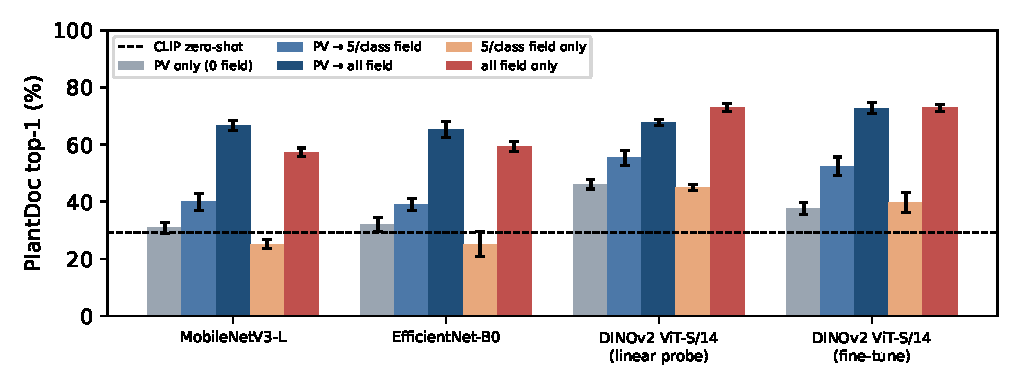
\includegraphics[width=0.66\linewidth]{../results/figures/field_labels.pdf}\hfill
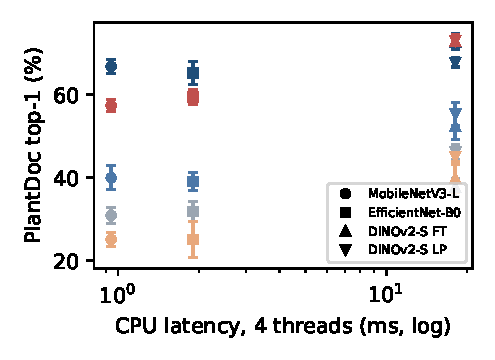
\includegraphics[width=0.32\linewidth]{../results/figures/acc_vs_latency.pdf}
\caption{\textbf{Left:} \PD top-1 by model and label regime (mean $\pm$ std over 3 seeds; dashed line: CLIP zero-shot). \textbf{Right:} the same points against measured CPU latency (ONNX Runtime, 4 threads, batch 1, log scale). Colors match the left panel. Latency for the linear probe equals that of the fine-tuned ViT.}
\label{fig:labels}
\end{figure*}

\begin{table*}[t]
\centering\small
\begin{tabular}{lccccc}\toprule
Model & PV only (0 field) & PV $\rightarrow$ 5/class field & PV $\rightarrow$ all field & 5/class field only & all field only \\\midrule
MobileNetV3-L & 30.9 $\pm$ 1.9 & 40.0 $\pm$ 2.9 & 66.8 $\pm$ 1.8 & 25.1 $\pm$ 1.6 & 57.3 $\pm$ 1.5 \\
EfficientNet-B0 & 31.9 $\pm$ 2.4 & 39.1 $\pm$ 2.1 & 65.3 $\pm$ 2.8 & 25.1 $\pm$ 4.3 & 59.5 $\pm$ 1.8 \\
DINOv2 ViT-S/14 (linear probe) & 46.2 $\pm$ 1.7 & 55.4 $\pm$ 2.7 & 67.8 $\pm$ 1.1 & 45.1 $\pm$ 1.1 & 73.0 $\pm$ 1.4 \\
DINOv2 ViT-S/14 (fine-tune) & 37.7 $\pm$ 2.2 & 52.4 $\pm$ 3.3 & 72.7 $\pm$ 2.0 & 39.8 $\pm$ 3.5 & 72.9 $\pm$ 1.1 \\
\bottomrule\end{tabular}

\caption{\textbf{\PD top-1 vs.\ field labels.} ``PV$\rightarrow$'' starts from the \PV-trained model of the same seed. ``only'' starts from generic pretrained weights. Mean $\pm$ std over 3 seeds. The de-duplicated variant is in \texttt{results/summary.md}.}
\label{tab:labels}
\end{table*}

\paragraph{Lab models fail first at recognizing the crop.}
Because each class is a (crop, condition) pair, we can split errors into two kinds (\cref{tab:errors}).
Lab-trained CNNs pick the wrong \emph{crop} for nearly half of the field images (crop accuracy \CropAccMnv--\CropAccEff\%). Given the right crop, they pick the exact class only \ClassGivenCropEff--\ClassGivenCropMnv\% of the time.
Most of the frozen DINOv2 probe's advantage is in crop recognition (\CropAccLP\%). Its class accuracy given the right crop (\ClassGivenCropLP\%) is close to the CNNs'.
Healthy-vs.-diseased accuracy is 82--87\% for lab-only models, against a majority-class baseline of \HealthyMajority\%.
In other words, the field failure is not only about subtle lesion appearance. Lab models also fail to recognize the plant itself in cluttered scenes.
This analysis was added after the main results were in, so it is exploratory.

\begin{table}[t]
\centering\scriptsize\setlength{\tabcolsep}{3pt}
\resizebox{\linewidth}{!}{\begin{tabular}{llccc}\toprule
Model & Regime & Crop & Class$\mid$crop & Healthy? \\\midrule
MobileNetV3-L & PV only & 53.8 & 57.5 & 83.9 \\
MobileNetV3-L & PV$\rightarrow$all & 83.9 & 79.6 & 94.9 \\
EfficientNet-B0 & PV only & 55.9 & 57.2 & 82.3 \\
EfficientNet-B0 & PV$\rightarrow$all & 83.8 & 77.9 & 93.4 \\
DINOv2 (linear probe) & PV only & 74.6 & 61.9 & 86.9 \\
DINOv2 (linear probe) & PV$\rightarrow$all & 90.1 & 75.2 & 93.2 \\
DINOv2 (fine-tune) & PV only & 64.8 & 58.2 & 84.5 \\
DINOv2 (fine-tune) & PV$\rightarrow$all & 91.0 & 80.0 & 96.0 \\
\bottomrule\end{tabular}
}
\caption{\textbf{Error decomposition on \PD test} (mean over 3 seeds, \%). Crop: predicted crop is correct. Class$\mid$crop: exact class correct among images with the correct crop. Healthy?: healthy-vs.-diseased correct (majority baseline \HealthyMajority\%).}
\label{tab:errors}
\end{table}

\paragraph{Five field images per class are not enough (C3 falsified).}
With 5 \PD images per class on top of \PV training, accuracy rises by 7--15 points (\cref{tab:labels}, \cref{fig:labels}). That recovers only \effbzeroRec\% (EfficientNet-B0), \mnvthreeRec\% (MobileNetV3) and \dinovtwoslpRec\% (both DINOv2 variants) of the gap between PV-only and PV$\rightarrow$all. This falls short of the 50\% we pre-registered.
For a practitioner, a few labeled field photos per disease help, but they are not a substitute for a real field training set.

\paragraph{Whether lab data helps depends on the model and the label budget.}
In the 5-per-class regime, starting from \PV is clearly better for every model, by +10 to +15 points (\cref{tab:paired}).
With all \PD training labels, \PV pretraining still helps both CNNs (MobileNetV3 \PCe, EfficientNet-B0 \PCg\ points). It makes no difference for fine-tuned DINOv2 (\PCk, CI [\PCklo, \PCkhi]), and it \emph{hurts} the frozen DINOv2 probe (\PCi, CI [\PCilo, \PCihi]).
For the probe, the explanation is narrow by construction. Its backbone is frozen and identical in both arms, so \PV enters \emph{only} through the starting point of the linear head. A head fitted to lab images is a useful prior when field labels are scarce (+10 points at 5/class). With all field labels, under our fixed schedule of 15 epochs, it ends up worse than a freshly initialized head.
For fine-tuned DINOv2, where the backbone does change, \PV pretraining is neutral once all field labels are available.
The best \PD accuracy overall (\dinovtwoslppdallpre\%) comes from the frozen DINOv2 probe trained on field data alone.

\begin{table}[t]
\centering\scriptsize\setlength{\tabcolsep}{2pt}
\resizebox{\linewidth}{!}{\begin{tabular}{lcc}\toprule
Comparison (A vs.\ B) & A$-$B & 95\% CI \\\midrule
DINOv2-LP vs EfficientNet-B0 (PV only) & +14.3 & [+8.2, +20.2] \\
DINOv2-LP vs DINOv2-FT (PV only) & +8.5 & [+3.1, +13.6] \\
DINOv2-LP (PV only) vs CLIP zero-shot & +16.9 & [+8.1, +25.3] \\
MobileNetV3-L: PV$\rightarrow$5/class vs 5/class only & +14.8 & [+10.7, +19.1] \\
MobileNetV3-L: PV$\rightarrow$all vs all field only & +9.5 & [+5.6, +13.3] \\
EfficientNet-B0: PV$\rightarrow$5/class vs 5/class only & +14.0 & [+10.2, +17.9] \\
EfficientNet-B0: PV$\rightarrow$all vs all field only & +5.8 & [+2.3, +9.3] \\
DINOv2 (linear probe): PV$\rightarrow$5/class vs 5/class only & +10.3 & [+5.6, +14.8] \\
DINOv2 (linear probe): PV$\rightarrow$all vs all field only & -5.2 & [-8.8, -2.0] \\
DINOv2 (fine-tune): PV$\rightarrow$5/class vs 5/class only & +12.6 & [+8.3, +16.9] \\
DINOv2 (fine-tune): PV$\rightarrow$all vs all field only & -0.1 & [-3.1, +3.0] \\
\bottomrule\end{tabular}
}
\caption{\textbf{Paired comparisons} on \PD test (seed-averaged top-1 difference in points, A$-$B; 95\% paired bootstrap CI over test images, 5{,}000 resamples, no multiple-comparison correction). LP/FT = DINOv2 linear probe / fine-tune.}
\label{tab:paired}
\end{table}

\paragraph{Edge cost (C4 falsified).}
\cref{tab:edge} reports cost on a desktop CPU (\EdgeCPU) and the RTX 5080.
The CNNs run in about 1--2\,ms per image with 4 CPU threads; DINOv2 ViT-S needs \CPUfourDino\,ms (\CPUoneDino\,ms single-threaded) and is about $5\times$ larger.
Our pre-registered C4 asked for a configuration within 5 points of the best accuracy at under 15\,ms. No configuration meets it. The fast CNNs peak at \mnvthreepdallinit\% (MobileNetV3, PV$\rightarrow$all), just below the 68.0\% threshold. The accurate DINOv2 models narrowly miss the latency limit, and the gap would widen on actual field hardware.
In practice the trade-off is mild in absolute terms: MobileNetV3 gives up about 6 points relative to the best model, in exchange for roughly $20\times$ lower CPU latency.

\begin{table}[t]
\centering\scriptsize\setlength{\tabcolsep}{2pt}
\resizebox{\linewidth}{!}{\begin{tabular}{lcccccc}\toprule
Model & Params (M) & ONNX (MB) & CPU-1 (ms) & CPU-4 (ms) & GPU (ms) & GPU mem (MB) \\\midrule
MobileNetV3-L & 4.2 & 16.1 & 2.7 & 0.9 & 3.53 & 40 \\
EfficientNet-B0 & 4.0 & 15.3 & 5.3 & 1.9 & 4.21 & 40 \\
DINOv2 ViT-S/14 & 21.6 & 82.4 & 51.8 & 18.1 & 2.76 & 139 \\
\bottomrule\end{tabular}
}
\caption{\textbf{Inference cost} at batch 1, $224\times224$: median over 300 runs after 50 warm-up runs. CPU: ONNX Runtime with 1 or 4 threads. GPU: PyTorch bf16. Params include the 28-way head.}
\label{tab:edge}
\end{table}

\paragraph{Seed noise vs.\ test noise (C5 holds, narrowly).}
Seed std on \PD reaches \effbzeroSeedSD\ points (EfficientNet-B0), just above our 2-point threshold. The per-run bootstrap interval half-width (\CIhwMin--\CIhwMax\ points) is about three times larger.
Seed averaging therefore stabilizes \emph{model} estimates, but it cannot fix a 236-image test set. Comparisons that differ by less than about 5 points on this split should be treated as ties unless a paired test says otherwise.

\section{Ablations and Robustness Checks}
\label{sec:ablations}

\paragraph{Is ``frozen beats fine-tuned'' a learning-rate artifact?}
All hyperparameters were fixed in advance, so a reviewer could reasonably suspect that the DINOv2 fine-tuning learning rate ($5\times10^{-5}$) was simply poorly chosen.
After the main results were in, we re-ran PV-only fine-tuning at $10^{-5}$ and $2\times10^{-4}$ (3 seeds each). This was a robustness check only and was not used to select any model (\cref{tab:sens}).
In-domain accuracy is essentially flat (99.4--99.5\%) across the 20$\times$ range. Field accuracy falls steadily as the learning rate rises, and every fine-tuned setting stays below the frozen probe.
This supports the reading that fine-tuning on lab images trades away transferable features, rather than reflecting one bad hyperparameter.

\begin{table}[t]
\centering\scriptsize
\begin{tabular}{lcc}\toprule
DINOv2-S, PV only & PV & PD \\\midrule
FT, lr 1e-5 & 99.5 $\pm$ 0.0 & 39.7 $\pm$ 1.4 \\
FT, lr 5e-5 (default) & 99.5 $\pm$ 0.1 & 37.7 $\pm$ 2.2 \\
FT, lr 2e-4 & 99.4 $\pm$ 0.0 & 29.9 $\pm$ 1.3 \\
LP, lr 1e-3 & 97.6 $\pm$ 0.1 & 46.2 $\pm$ 1.7 \\
\bottomrule\end{tabular}

\caption{\textbf{DINOv2 ViT-S, trained on \PV only:} fine-tuning learning rate vs.\ in-domain (PV) and field (PD) top-1. Mean $\pm$ std over 3 seeds. The check was run after the main results and was not used for selection.}
\label{tab:sens}
\end{table}

\paragraph{Test-set de-duplication.}
Removing the \PDdups \PD test images that near-duplicate \PD training images changes source-only accuracies by under one point (\cref{tab:source}). It changes the regimes trained on \PD by up to about 2 points, most for fine-tuned DINOv2 with all field labels (72.7$\rightarrow$75.0; full table in \texttt{results/summary.md}).
Accuracy mostly goes \emph{up} after removal, so on this split the duplicates did not inflate results. None of our conclusions change on the de-duplicated set. We still recommend reporting it, because the effect could differ for other models or splits.

\paragraph{Lab pretraining as initialization.}
The PV$\rightarrow$ vs.\ ``only'' columns of \cref{tab:labels} are themselves an ablation of the \PV stage. The paired results in \cref{tab:paired} show that the \PV stage is worth +10 to +15 points with 5 field images per class for every model. With all field labels it is worth less for the CNNs, nothing for fine-tuned DINOv2, and is harmful for the frozen probe. For the probe, the \PV stage only sets the head's initialization, because the backbone is frozen in both arms.

\section{Limitations and Broader Impact}
\label{sec:limits}

\paragraph{Statistical power.}
The \PD test set has only \PDtestN images (4--12 per class). \emph{Tomato two-spotted spider mites} has no test images and only 2 training images, so in the 5/class regime it contributes 2 images. Bootstrap intervals are therefore several points wide (\cref{tab:source}). Differences smaller than that should not be read as rankings. That is the reason we pre-registered thresholds and report intervals rather than bolding the best number.

\paragraph{One target domain, one image type.}
\PD is a single web-scraped field dataset of mostly single-leaf or few-leaf photos. Its photographers, devices, regions and seasons are unknown, so ``field'' here means \emph{uncontrolled imagery}, not a specific farm, crop season or sensor. Results may not transfer to drone, multispectral, or canopy-level imagery, or to growing regions under-represented in both datasets. The label space covers 13 crops (apple, bell pepper, blueberry, cherry, corn, grape, peach, potato, raspberry, soybean, squash, strawberry, tomato). Many staple crops, such as cassava, rice and wheat, are absent.

\paragraph{Label noise and leakage.}
\PD labels come from web image search and have not been re-verified by pathologists. Our near-duplicate check uses only perceptual hashing, so it may miss crops or edits of the same photo. Several \PD classes are \emph{healthy} leaves of different crops, so part of the task is crop identification rather than disease diagnosis.

\paragraph{Compute and tuning.}
To stay within a 5\,GPU-hour budget, all hyperparameters were fixed in advance and never tuned. Every model might improve with tuning, especially DINOv2 fine-tuning, which is sensitive to learning rate. Our latency numbers come from a desktop CPU, not a phone or microcontroller; they bound relative cost but do not give absolute on-device timings.

\paragraph{Broader impact.}
A classifier that scores 99\% in the lab and far lower in the field can do real harm if it is deployed on the strength of the lab number: missed infections, or unneeded pesticide applications. Our main recommendation is procedural. Report field-domain accuracy with intervals, publish label maps, and de-duplicate test sets before claiming deployability. Any tool built on these models should present predictions as decision support for growers and extension agents, with explicit uncertainty, not as a diagnosis. Both datasets are public and contain no personal data. PlantVillage is CC BY-SA 3.0 and PlantDoc is CC BY 4.0; we redistribute no images.

\section{Conclusion}
\label{sec:conclusion}

We measured the PlantVillage$\rightarrow$PlantDoc shift with a seeded, released protocol on a single consumer GPU in \GPUHours\ GPU-hours.
Lab accuracy says almost nothing about field accuracy: every model loses at least \dinovtwoslpGap\ points.
Three results seem practically useful. A frozen, generic self-supervised backbone is the best starting point when no field labels exist. A handful of field labels helps but recovers well under half of the gap. And lab pretraining reliably helps small CNNs, but for a foundation backbone it pays off only when field labels are scarce.
Two of our five pre-registered claims were falsified, and we report them as such.
Finally, with a \PDtestN-image test set the field-domain evaluation itself is the bottleneck. We encourage future lab-to-field work to report paired intervals, publish label maps, de-duplicate test sets, and move toward larger in-the-wild test sets such as PlantWild~\cite{wei2024benchmarking}.

{
    \small
    \bibliographystyle{ieeenat_fullname}
    \bibliography{../refs/verified}
}
\end{document}
